Servlet- tai FastCGI-tekniikka ei sido web-sovelluksen arkkitehtuuria, vaan molempia tekniikoita käytettäessä sovellusten perusarkkitehtuuri on sama. Sovellukset ovat jatkuvasti käynnissä olevia prosesseja, joille käyttäjän syöttämän datan lisäksi allokoidaan joukko erilaisia suoritusympäristöön liittyviä resursseja ja muuttujia (mm. tietokantayhteys) \cite{uml}. Syötteen perusteella sovellus tuottaa tulosteen, joka palautetaan käyttäjälle.

Tyypillinen tapa toteuttaa web-sovelluksia nykypäivänä on käyttää sovelluskehystä, mikä tuo oman lisänsä sovellusten arkkitehtuuriin. Yleisesti käytettyjä web-sovelluskehyksiä ovat esimerkiksi Javalla toteutettu Spring, Pythonilla tehty Django ja Ruby-ohjelmointikieleen perustuva Ruby on Rails \cite{spring, django, ruby2011agile}. Näissä sovelluskehyksissä erillinen viestinvälittäjä (dispatcher) ottaa vastaan pyynnön ja välittää sen eteenpäin. Pyyntö ei siirry suoraan sovellusohjelmalle, vaan se välitetään väliohjelma-kerroksen läpi kuvassa \ref{dispatcher} esitetyllä tavalla. Nämä väliohjelmat esimerkiksi tekevät merkintöjä lokitiedostoihin, asettavat ja lukevat käyttäjän selaimen evästeitä tai asettavat ympäristömuuttujia sovellusohjelmaa varten.

\begin{figure}[h]
\centering
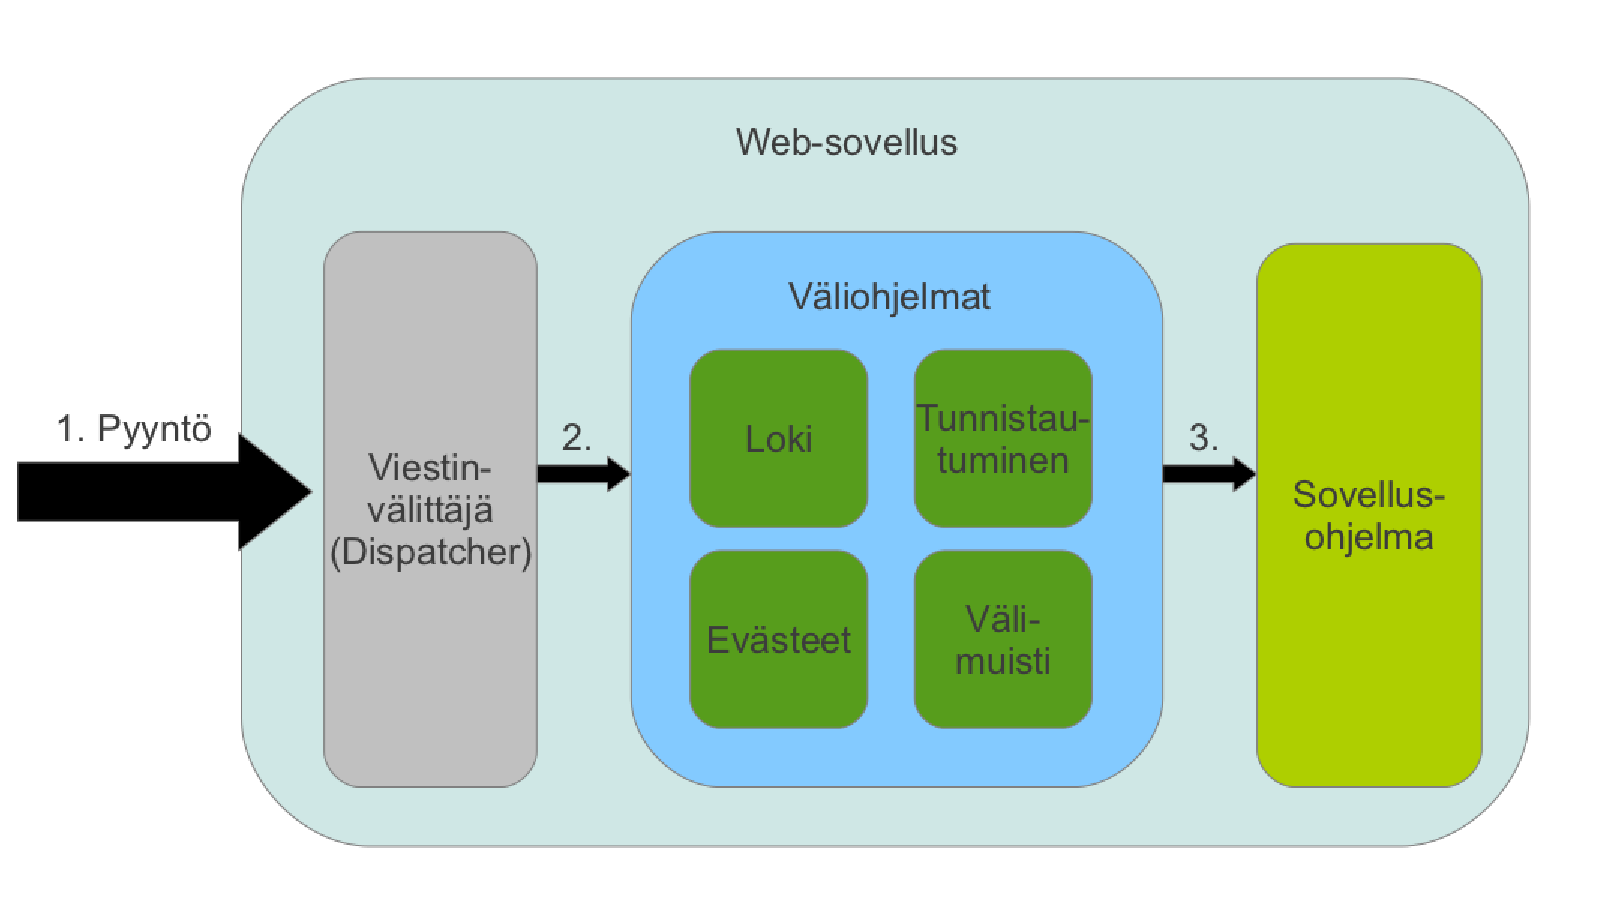
\includegraphics[width=\textwidth]{web/dispatcher.eps}
\caption{Web-sovelluskehyksellä toteutetun web-sovelluksen kontrollin kulku \cite{ruby2011agile}.}%
\label{dispatcher}
\end{figure}

Web-sovellusohjelmista on pyritty karsimaan paljon yleisiä tehtäviä. Ne on jätetty sovelluskehyksen tai käyttäjän toteuttaman väliohjelman tehtäväksi. Web-sovellus käyttää hyväkseen sovelluskehyksen tarjoamia parametreja, jotka ovat esimerkiksi viittauksia muuttujiin, joita säilytetään käyttäjän istunnon ajan muistissa. Myös käyttäjän tunnistaminen on yksi sovelluskehyksen tehtävistä \cite{ruby2011agile}. Tällöin sovellusohjelma saa ympäristömuuttujana kirjautuneen käyttäjän tiedot (esimerkiksi tunnistenumeron ja käyttöoikeudet), joita se voi käyttää hyväkseen ohjelmalogiikassaan.